\section{Mixed Cell Volume Radionuclide Model}\label{sec:mixed_cell}

    % WF : glass 

      % alteration

      % temperature limit

    % WF : uox 

      % cladding limit

      % corrosion

A main nuclide transport component model used in this work is a mixed cell 
component module incorporating solubility and sorption effects as well as  
engineered material dissolution.

A graphical representation of the mixed cell model is given in Figures 
\ref{fig:intact} and \ref{fig:dissolved}.  

\begin{figure}[h!]
\begin{minipage}[b]{0.5\linewidth}
  \begin{center}
    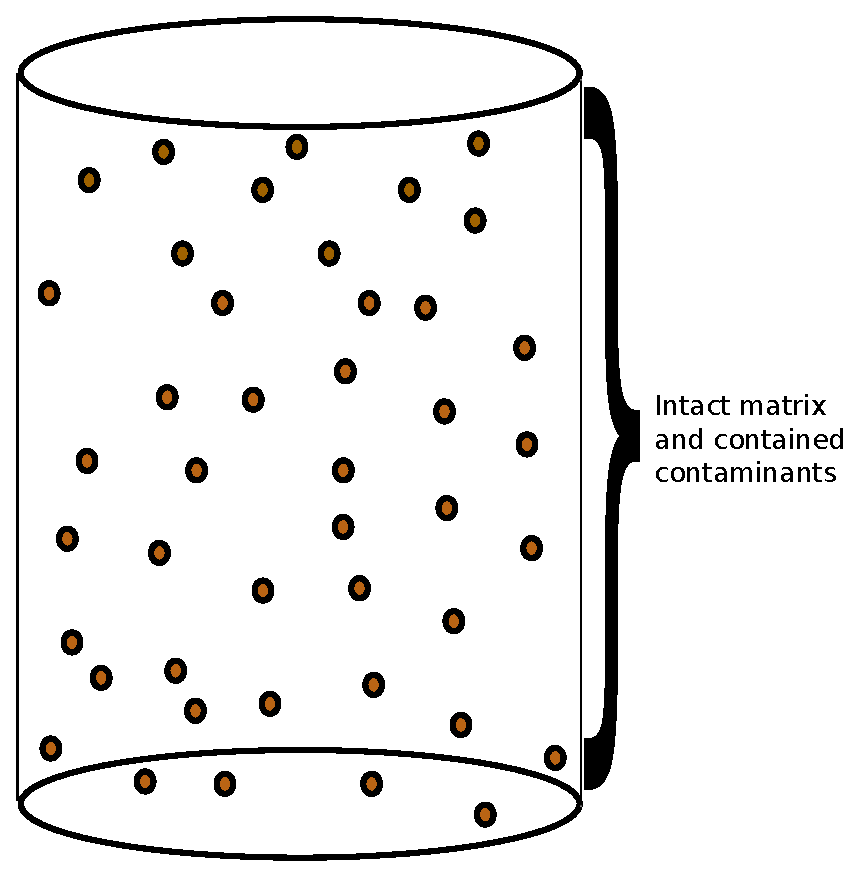
\includegraphics[height=7cm]{./chapters/nuclide_models/mixed_cell/mixed_cell_whole.eps}
  \end{center}
  \caption[Intact Mixed Cell Control Volume]{The control volume contains an 
  intact material matrix and contaminants that are unavailable to neighboring 
  subcomponents until dissolution has begun.}
  \label{fig:intact}
\end{minipage}
\hspace{0.5cm}
\begin{minipage}[b]{0.5\linewidth}
  \begin{center}
    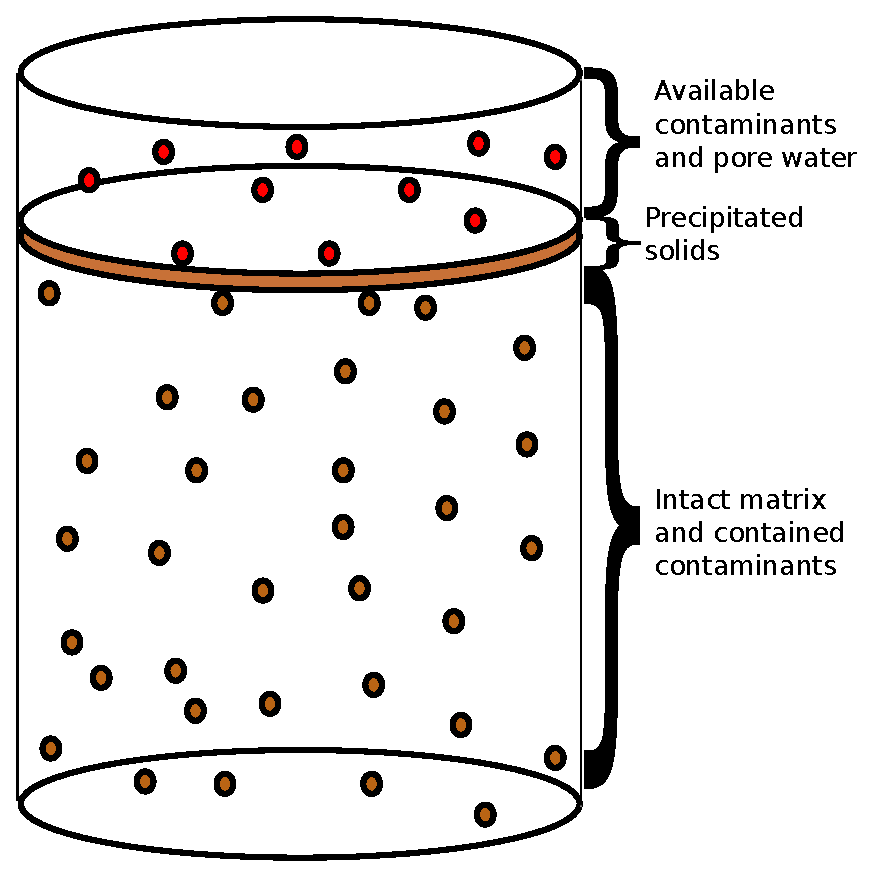
\includegraphics[height=7cm]{./chapters/nuclide_models/mixed_cell/mixed_cell_degraded.eps}
  \end{center}
  \caption[Degrading Mixed Cell Control Volume]{Once dissolution begins, the 
  :control volume contains a partially dissolved material matrix, contaminated 
  pore water, and precipitated solids.}
  \label{fig:dissolved}
\end{minipage}
\end{figure}


After some time degrading, the volume of free fluid can be expressed 
\begin{align}
V_{ff} &= \phi V_T \int_{t_0}^{t_n} f(\cdots) dt.
\label{vff}
\end{align}
The volume of the intact matrix can be expressed
\begin{align}
V_m &= V_T(1-\int_{t_0}^{t_n} f(\cdots) dt.
\label{vm}
\end{align}
Finally, the volume of the precipitated solids can be expressed
\begin{align}
V_{ps} &= V_T(1-\int_{t_0}^{t_n} f(\cdots) dt.
\label{vps}
\end{align}

The contaminant mass in the free fluid is just the pore water concentration 
times the free fluid volume plus the time integral of net influx to the cell. 
This model assumes that all net influx to the cell enters the free fluid rather 
than the intact matrix. The resulting expression for the contaminant mass in the 
free fluid is 

\begin{align}
m_{ff} &= C\phi V_T\int_{t_0}^{t_n}f(\cdots)dt\nonumber\\ 
       &= \left[C_0 + \frac{\int_{t_0}^{t_n} \dot{m}_{hi} dt}{\phi V_T\int_{t_0}^{t_n}f(\cdots)}\right] \phi V_T\int_{t_0}^{t_n}f(\cdots)dt 
\intertext{which, for discrete times becomes }
m_{ff} &= \left[C_0 + \frac{\sum_{p=1}^{n} \dot{m}_{hi} (t_p - t{p-1}) }{\phi V_T\sum_{p=1}^{n}f(\cdots)}\right] \phi V_T\sum_{p=1}^{n}f(\cdots)(t_p - t_{p-1})
\label{mff}
\end{align}



